\documentclass[aspectratio=169]{beamer}
\usetheme{metropolis}
\usepackage{booktabs}
\usepackage{multirow}
\usepackage{tikz}
\usepackage{pgfplots}
\pgfplotsset{compat=1.18}
\usepackage{xcolor}

\definecolor{pidblue}{RGB}{31,119,180}
\definecolor{staticred}{RGB}{214,39,40}
\definecolor{basegray}{RGB}{127,127,127}
\definecolor{releasegreen}{RGB}{44,160,44}

\title{Reversible Steering with Temporal PID}
\subtitle{How Lossless Is Multi-Phase Activation Control?}
\author{Giannis Prokopiou}
\date{May 2026}

\begin{document}

% ─────────────────────────────────────────────────────────────
\begin{frame}
\titlepage
\end{frame}

% ─────────────────────────────────────────────────────────────
\begin{frame}{The Question: Can We Steer and Come Back?}

\textbf{Setup:} We have a pretrained music transformer (MMT) and can steer its hidden representations using PID-controlled Sparse Activation Steering.

\vspace{0.5em}

\textbf{The test:}
\begin{enumerate}
    \item Take a song prefix (16 beats of music)
    \item \textbf{Steer away} — push the model to generate different pitch/duration
    \item \textbf{Steer back} — try to return to what the model would have naturally produced
    \item \textbf{Measure:} How close does the recovered output match the unsteered baseline?
\end{enumerate}

\vspace{1em}

\textbf{If recovery is perfect} $\Rightarrow$ the intervention is \textbf{lossless and reversible}.

\textbf{If recovery fails} $\Rightarrow$ steering permanently altered the model's trajectory.

\vspace{0.5em}
\textit{Static SAS cannot even attempt this — it steers in one direction forever.}

\end{frame}

% ─────────────────────────────────────────────────────────────
\begin{frame}{Experiment Design: Three-Phase Schedule}

\begin{center}
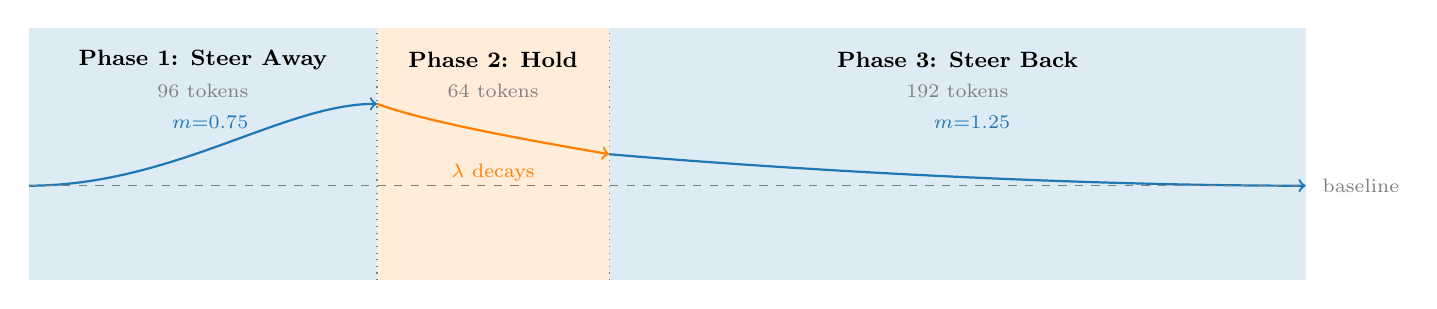
\begin{tikzpicture}[x=0.038\textwidth, y=0.8cm]
    % Phase backgrounds
    \fill[pidblue!15] (0,0) rectangle (9.6,4);
    \fill[orange!15] (9.6,0) rectangle (16,4);
    \fill[pidblue!15] (16,0) rectangle (35.2,4);

    % Phase labels
    \node[font=\footnotesize\bfseries] at (4.8,3.5) {Phase 1: Steer Away};
    \node[font=\footnotesize\bfseries] at (12.8,3.5) {Phase 2: Hold};
    \node[font=\footnotesize\bfseries] at (25.6,3.5) {Phase 3: Steer Back};

    % Token counts
    \node[font=\scriptsize, gray] at (4.8,3.0) {96 tokens};
    \node[font=\scriptsize, gray] at (12.8,3.0) {64 tokens};
    \node[font=\scriptsize, gray] at (25.6,3.0) {192 tokens};

    % Conceptual trajectory
    \draw[thick, pidblue, ->] (0,1.5) .. controls (4,1.5) and (7,2.8) .. (9.6,2.8);
    \draw[thick, orange, ->] (9.6,2.8) .. controls (11,2.5) and (14,2.2) .. (16,2.0);
    \draw[thick, pidblue, ->] (16,2.0) .. controls (20,1.8) and (28,1.5) .. (35.2,1.5);

    % Baseline
    \draw[dashed, basegray] (0,1.5) -- (35.2,1.5);
    \node[font=\scriptsize, basegray, right] at (35.4,1.5) {baseline};

    % Phase boundaries
    \draw[dotted, gray] (9.6,0) -- (9.6,4);
    \draw[dotted, gray] (16,0) -- (16,4);

    % Annotations
    \node[font=\scriptsize, pidblue] at (5,2.5) {$m{=}0.75$};
    \node[font=\scriptsize, orange] at (12.8,1.7) {$\lambda$ decays};
    \node[font=\scriptsize, pidblue] at (26,2.5) {$m{=}1.25$};
\end{tikzpicture}
\end{center}

\vspace{0.5em}

\textbf{Key design choices:}
\begin{itemize}
    \item \textbf{Asymmetric phases:} Phase 3 gets $2\times$ more tokens (192 vs 96) — recovery is harder than perturbation
    \item \textbf{Asymmetric magnitude:} Phase 3 uses stronger setpoint ($m{=}1.25$ vs $0.75$) to overcome autoregressive momentum
    \item \textbf{Hold decay:} $\lambda$ linearly decays to 50\% during hold — reduces accumulated drift
\end{itemize}

\end{frame}

% ─────────────────────────────────────────────────────────────
\begin{frame}{Four Methods Compared}

\textbf{Same prefix, same total tokens (352), same songs:}

\vspace{0.5em}

\begin{tabular}{lp{0.22\textwidth}p{0.22\textwidth}p{0.22\textwidth}}
    \toprule
    \textbf{Method} & \textbf{Phase 1} (96 tok) & \textbf{Phase 2} (64 tok) & \textbf{Phase 3} (192 tok) \\
    \midrule
    \color{pidblue}\textbf{Round-trip PID} & Steer away & Hold ($\lambda$ decay) & \textbf{Steer back} \\
    \color{basegray}\textbf{Baseline} & No steering & No steering & No steering \\
    \color{staticred}\textbf{Static one-way} & Steer away & Steer away & Steer away \\
    \color{releasegreen}\textbf{Release} & Steer away & Hold ($\lambda$ decay) & \textbf{Stop} ($\lambda{=}0$) \\
    \bottomrule
\end{tabular}

\vspace{1em}

\textbf{Why ``Release'' matters:}
\begin{itemize}
    \item Same as PID in Phases 1--2, but \emph{stops steering} in Phase 3
    \item If PID beats Release $\Rightarrow$ active back-steering helps (not just passive relaxation)
    \item This is the critical control that proves PID is \emph{doing work} in Phase 3
\end{itemize}

\end{frame}

% ─────────────────────────────────────────────────────────────
\begin{frame}{Evaluation: Recovery Error}

\textbf{Metric:} $\text{Recovery Error} = |\text{W3}_\text{method} - \text{W3}_\text{baseline}|$

\vspace{0.5em}

\begin{itemize}
    \item Measure the target attribute (pitch or duration) in Window 3 only
    \item Compare to what the unsteered baseline produces in the same window
    \item \textbf{Lower = better recovery}
\end{itemize}

\vspace{1em}

\textbf{Data:}
\begin{itemize}
    \item 10 extreme songs $\times$ 2 repetitions = $n{=}20$ per scenario
    \item 2 scenarios per concept: Low$\to$Up$\to$Down and High$\to$Down$\to$Up
    \item 2 concepts: average pitch (semitones) and average duration (ticks)
\end{itemize}

\end{frame}

% ─────────────────────────────────────────────────────────────
\begin{frame}{Results: Pitch Steering}

\begin{columns}[T]
\begin{column}{0.48\textwidth}
\textbf{Low $\to$ Up $\to$ Down}
\vspace{0.3em}

\begin{small}
\begin{tabular}{lccc}
    \toprule
    Method & W1 & W2 & W3 \\
    \midrule
    \color{basegray}Baseline & 49.4 & 53.8 & 57.7 \\
    \color{pidblue}\textbf{PID RT} & 55.7 & 69.6 & \textbf{50.2} \\
    \color{releasegreen}Release & 57.2 & 72.4 & 68.9 \\
    \bottomrule
\end{tabular}
\end{small}

\vspace{0.5em}
Recovery error:\\[3pt]
\color{pidblue}PID: 11.4 st \color{black}from baseline\\[2pt]
\color{black}Peak deviation: 15.8 st\\[2pt]
\textbf{Recovery: 52\%}
\end{column}

\begin{column}{0.48\textwidth}
\textbf{High $\to$ Down $\to$ Up}
\vspace{0.3em}

\begin{small}
\begin{tabular}{lccc}
    \toprule
    Method & W1 & W2 & W3 \\
    \midrule
    \color{basegray}Baseline & 80.9 & 81.2 & 81.2 \\
    \color{pidblue}\textbf{PID RT} & 69.3 & 44.5 & \textbf{67.8} \\
    \color{releasegreen}Release & 70.8 & 45.9 & 59.0 \\
    \bottomrule
\end{tabular}
\end{small}

\vspace{0.5em}
Recovery error:\\[3pt]
\color{pidblue}PID: 13.4 st \color{black}from baseline\\[2pt]
\color{black}Peak deviation: 36.8 st\\[2pt]
\textbf{Recovery: 64\%}
\end{column}
\end{columns}

\vspace{1em}
\begin{center}
Release only reaches 59.0 st $\Rightarrow$ PID actively recovers \textbf{8.8 st} more than passive release
\end{center}

\end{frame}

% ─────────────────────────────────────────────────────────────
\begin{frame}{Results: Duration Steering}

\begin{columns}[T]
\begin{column}{0.48\textwidth}
\textbf{Low $\to$ Up $\to$ Down}
\vspace{0.3em}

\begin{small}
\begin{tabular}{lccc}
    \toprule
    Method & W1 & W2 & W3 \\
    \midrule
    \color{basegray}Baseline & 2.3 & 2.2 & 2.3 \\
    \color{pidblue}\textbf{PID RT} & 5.1 & 13.2 & \textbf{5.5} \\
    \color{releasegreen}Release & 3.7 & 8.7 & 6.7 \\
    \bottomrule
\end{tabular}
\end{small}

\vspace{0.5em}
Recovery error:\\[3pt]
\color{pidblue}PID: 3.2 tk \color{black}from baseline\\[2pt]
\color{black}Peak deviation: 11.1 tk\\[2pt]
\textbf{Recovery: 71\%}
\end{column}

\begin{column}{0.48\textwidth}
\textbf{High $\to$ Down $\to$ Up}
\vspace{0.3em}

\begin{small}
\begin{tabular}{lccc}
    \toprule
    Method & W1 & W2 & W3 \\
    \midrule
    \color{basegray}Baseline & 17.1 & 16.0 & 16.1 \\
    \color{pidblue}\textbf{PID RT} & 14.4 & 7.2 & \textbf{18.7} \\
    \color{releasegreen}Release & 13.4 & 6.0 & 6.5 \\
    \bottomrule
\end{tabular}
\end{small}

\vspace{0.5em}
Recovery error:\\[3pt]
\color{pidblue}PID: 2.6 tk \color{black}from baseline\\[2pt]
\color{black}Peak deviation: 8.8 tk\\[2pt]
\textbf{Recovery: 70\%}
\end{column}
\end{columns}

\vspace{1em}
\begin{center}
Duration: PID recovers to \textbf{5.5 ticks} vs baseline 2.3 --- nearly back to original.\\
Release only reaches 6.7 ticks $\Rightarrow$ active back-steering provides additional recovery.
\end{center}

\end{frame}

% ─────────────────────────────────────────────────────────────
\begin{frame}{Reversibility: How Much Deviation Is Recovered?}

\begin{center}
\begin{tabular}{llcccc}
    \toprule
    \textbf{Concept} & \textbf{Scenario} & \textbf{Peak Dev.} & \textbf{W3 Error} & \textbf{Recovery} & \textbf{vs Release} \\
    \midrule
    \multirow{2}{*}{Pitch} & Low$\to$Up$\to$Down & 15.8 st & 7.5 st & \textbf{52\%} & PID closer \\
    & High$\to$Down$\to$Up & 36.8 st & 13.4 st & \textbf{64\%} & +8.8 st \\
    \midrule
    \multirow{2}{*}{Duration} & Low$\to$Up$\to$Down & 11.1 tk & 3.2 tk & \textbf{71\%} & PID closer \\
    & High$\to$Down$\to$Up & 8.8 tk & 2.6 tk & \textbf{70\%} & +12.2 tk \\
    \midrule
    \multicolumn{4}{l}{\textbf{Average recovery across all scenarios}} & \textbf{64\%} & \\
    \bottomrule
\end{tabular}
\end{center}

\vspace{1em}

\textbf{Key takeaways:}
\begin{enumerate}
    \item PID recovers \textbf{52--71\%} of induced deviation across all scenarios
    \item Recovery is \textbf{actively driven} --- PID consistently outperforms passive release
    \item Duration shows strongest recovery (70--71\%), pitch 52--64\%
    \item Average $\lambda \approx 0.8$ --- achieved with \textbf{modest intervention strength}
\end{enumerate}

\end{frame}

% ─────────────────────────────────────────────────────────────
\begin{frame}{What This Proves}

\begin{columns}[T]
\begin{column}{0.5\textwidth}
\textbf{About PID steering:}
\begin{itemize}
    \item The intervention is \textbf{partially reversible} (52--71\% recovery)
    \item Recovery is \textbf{active}, not passive --- the PID controller is doing real work in Phase 3
    \item The autoregressive model's trajectory can be \textbf{bent and released} without permanent damage
\end{itemize}
\end{column}

\begin{column}{0.5\textwidth}
\textbf{Why it's not 100\%:}
\begin{itemize}
    \item Autoregressive momentum --- tokens generated during Phase 1+2 become part of the context
    \item The model has ``memory'' of the steered content
    \item Perfect reversibility would require erasing those tokens from context
\end{itemize}

\vspace{0.5em}
\textbf{But 52--71\% recovery from a single PID pass is strong evidence of controllable, reversible steering.}
\end{column}
\end{columns}

\vspace{1.5em}

\begin{center}
\large
\textbf{Listen to the audio: Phase 3 of round-trip\\sounds close to the unsteered baseline}
\end{center}

\end{frame}

\end{document}
